\documentclass[12pt]{article}
\usepackage{latexsym,amssymb,amsmath} % for \Box, \mathbb, split, etc.
% \usepackage[]{showkeys} % shows label names
\usepackage{cite} % sorts citation numbers appropriately
\usepackage{path}
\usepackage{url}
\usepackage{verbatim}
\usepackage[pdftex]{graphicx}

% horizontal margins: 1.0 + 6.5 + 1.0 = 8.5
\setlength{\oddsidemargin}{0.0in}
\setlength{\textwidth}{6.5in}
% vertical margins: 1.0 + 9.0 + 1.0 = 11.0
\setlength{\topmargin}{0.0in}
\setlength{\headheight}{12pt}
\setlength{\headsep}{13pt}
\setlength{\textheight}{625pt}
\setlength{\footskip}{24pt}

\renewcommand{\textfraction}{0.10}
\renewcommand{\topfraction}{0.85}
\renewcommand{\bottomfraction}{0.85}
\renewcommand{\floatpagefraction}{0.90}

\usepackage{accents}
\newcommand{\ubar}[1]{\underaccent{\bar}{#1}}
\makeatletter
\setlength{\arraycolsep}{2\p@} % make spaces around "=" in eqnarray smaller
\makeatother
\usepackage{stackengine}
% change equation, table, figure numbers to be counted inside a section:
\numberwithin{equation}{section}
\numberwithin{table}{section}
\numberwithin{figure}{section}

% begin of personal macros
\newcommand{\half}{{\textstyle \frac{1}{2}}}
\newcommand{\eps}{\varepsilon}
\newcommand{\myth}{\vartheta}
\newcommand{\myphi}{\varphi}

\newcommand{\IN}{\mathbb{N}}
\newcommand{\IZ}{\mathbb{Z}}
\newcommand{\IQ}{\mathbb{Q}}
\newcommand{\IR}{\mathbb{R}}
\newcommand{\IC}{\mathbb{C}}
\newcommand{\Real}[1]{\mathrm{Re}\left({#1}\right)}
\newcommand{\Imag}[1]{\mathrm{Im}\left({#1}\right)}
\DeclareRobustCommand{\brkbinom}{\genfrac[]{0pt}{}}
\newcommand{\norm}[2]{\|{#1}\|_{{}_{#2}}}
\newcommand{\abs}[1]{\left|{#1}\right|}
\newcommand{\ip}[2]{\left\langle {#1}, {#2} \right\rangle}
\newcommand{\der}[2]{\frac{\partial {#1}}{\partial {#2}}}
\newcommand{\dder}[2]{\frac{\partial^2 {#1}}{\partial {#2}^2}}
\usepackage{enumitem}
\newcommand{\nn}{\mathbf{n}}
\newcommand{\xx}{\mathbf{x}}
\newcommand{\uu}{\mathbf{u}}
\usepackage{tikz}
\usetikzlibrary{arrows}
\usetikzlibrary{positioning}
\usepackage{titlesec}
\newcommand{\junk}[1]{{}}
\usepackage{sectsty}
\usepackage{xcolor}
\newcommand*{\bfrac}[2]{\genfrac{}{}{0pt}{}{#1}{#2}}
\newcommand\myatop[2]{\left[{{#1}\atop#2}\right]} % "wrapper macro"
\usepackage{array}
\usepackage{multirow}
\usepackage{amsmath}
\DeclareMathOperator*{\argmax}{arg\,max}
\DeclareMathOperator*{\argmin}{arg\,min}
\makeatletter
\renewcommand*\env@matrix[1][\arraystretch]{%
	\edef\arraystretch{#1}%
	\hskip -\arraycolsep
	\let\@ifnextchar\new@ifnextchar
	\array{*\c@MaxMatrixCols c}}
\makeatother

\makeatletter
\renewcommand*\env@matrix[1][*\c@MaxMatrixCols c]{%
	\hskip -\arraycolsep
	\let\@ifnextchar\new@ifnextchar
	\array{#1}}
\makeatother

\definecolor{darkblue}{rgb}{0,0,0.4}
\usepackage[colorlinks = true,
linkcolor = darkblue,
urlcolor  = darkblue,
citecolor = darkblue,
anchorcolor = darkblue]{hyperref}
% set two lengths for the includegraphics commands used to import the plots:
\newlength{\fwtwo} \setlength{\fwtwo}{0.45\textwidth}
% end of personal macros

\begin{document}
\DeclareGraphicsExtensions{.jpg}

\begin{center}
\textsc{\Large Statistical Pattern Recognition} \\[2pt]
	\textsc{\large Assignment 5}\\
	\vspace{0.5cm}
  Ali Gholami \\[6pt]
  Department of Computer Engineering \& Information Technology\\
  Amirkabir University of Technology  \\[6pt]
  \def\UrlFont{\em}
  \url{https://aligholamee.github.io}\\
    \href{mailto:aligholami7596@gmail.com}{\textit{aligholami7596@gmail.com}}
\end{center}

\begin{abstract}

\end{abstract}

\subparagraph{Keywords.} \textit{Dimensionality Reduction, Principal Component Analysis, Fisher Linear Discriminant Analysis, Feature Subset Selection, Sequential Feature Selection, Data Visualization \& Representation.}


\section{Sequential Feature Selection}
Given the following objective function, use \textbf{SFS}, \textbf{SBS} and \textbf{Plus-2 Minus-1 Selection} to select 3 features:
$$
	J(x) = 5x_1 + 7x_2 + 4x_3 + 9x_4 + 3x_5 -2x_1x_2 + 2x_1x_2x_3 - 2x_2x_3 - 4x_1x_2x_3x_4 + 3x_1x_3x_5
$$
\subsection*{Solution}
\subsubsection*{SFS}
In this method, we start feature selection from an empty set. We add features one by one and compute the value of the objective function with respect to each of the features being added. The feature with the largest objective function will be selected. The iteration goes on until all features all covered. We then select ideal features (subset with k features and maximum objective). The actual algorithm is as following:
\begin{enumerate}
	\item Start with the empty set $ Y_0 = \emptyset$
	\item Select the next best feature $ x^+ = argmax[J(Y_k + x)]$
	\item Update $Y_{k + 1} = Y_k + x^+;\ \ k = k + 1$
	\item Go to 2
\end{enumerate}
Below is the demonstration of iterations taken to completely explore the search space. The first iteration is:
\begin{itemize}
	\item $J(x_1) = 5$
	\item $J(x_2) = 7$
	\item $J(x_3) = 4$
	\item $J(x_4) = 9$
	\item $J(x_5) = 3$
\end{itemize}
According to the heuristic nature of sequential subset selection, we'll choose $x_4$ as the first best feature. We'll then generate subsets containing combination of features with $x_4$:
\begin{itemize}
	\item $J(x_4x_1) = 14$
	\item $J(x_4x_2) = 16$
	\item $J(x_4x_3) = 13$
	\item $J(x_4x_5) = 12$
\end{itemize}
Thus, features $x_4$ and $x_2$ are selected until now. We'll drive the 3 sized subsets:
\begin{itemize}
	\item $J(x_4x_2x_1) = 19$
	\item $J(x_4x_2x_3) = 18$
	\item $J(x_4x_2x_5) = 22$
\end{itemize}
Three best features selected by the algorithm are $x_4$, $x_2$ and $x_5$.

\subsubsection*{SBS}
This method initiates the feature selection procedure using a complete subset of features. It then removes each feature and evaluates the objective function. The feature that causes the lowest decrease in the objective function will be remove (useless feature!). We'll stop when we reach a satisfying 3 sized feature subset. The algorithm is formally working as follows:
\begin{enumerate}
	\item Start with the full set $ Y_0 = X$
	\item Remove the worst feature $x^- = argmax[J(Y_k - x)]$
	\item Update $Y_{k + 1} = Y_{k} - x^-;\ \ k = k + 1 $
	\item Go to 2
\end{enumerate}
Applying this algorithm on the given objective function yields the following results:
\begin{itemize}
	\item $J(x_1x_2x_3x_4x_5) = 25$
\end{itemize}
And the results of removing each of the features:
\begin{itemize}
	\item $J(x_1x_2x_3x_4) = 19$
	\item $J(x_1x_2x_3x_5) = 20$
	\item $J(x_1x_2x_4x_5) = 22$
	\item $J(x_1x_3x_4x_5) = 24$
	\item $J(x_2x_3x_4x_5) = 21$
\end{itemize}
It is obvious that $x_2$ is the most useless feature among these. We'll remove $x_2$ and obtain the feature subset with 4 features: $x_1$, $x_3$, $x_4$ and $x_5$.
\begin{itemize}
	\item $J(x_1x_3x_4x_5) = 24$
\end{itemize}
We can obtain the following subsets:
\begin{itemize}
	\item $J(x_1x_3x_4) = 18$
	\item $J(x_1x_3x_5) = 15$
	\item $J(x_1x_4x_5) = 17$
	\item $J(x_3x_4x_5) = 16$
\end{itemize}
$x_5$ will be removed since it has the lowest effect on the greatness of evaluation.
The proper feature subset includes: $x_1$, $x_3$ and $x_4$.

\section{PCA \& FLDA}
In this problem, dimensionality reduction with a two-feature two-class dataset is explored. Consider the following dataset and the test sample: $x = [0.85\ \ \ 1.15]^T$
\begin{itemize}
	\item 	\textbf{Class 1}: [[0.8, 1.2], [0.9, 1.4], [1.2, 1.4], [1.1, 1.5]]
	\item \textbf{Class 2}: [[0.8, 1.1], [0.6, 1], [0.65, 1.1], [0.75, 0.9]]
\end{itemize}
\begin{enumerate}[label=(\alph*)]
	\item Demonstrate the preprocessing steps (need to show step-by-step details). Calculate the \textbf{mean} of each class ($m_1$ and $m_2$). Calculate the \textbf{covariance} matrix of each class.
	
	\item Using \textbf{Fisher's Linear Discriminant} to find a projection vector (w) which optimally separates the projections of these two classes.
	
	\item Is the vector derived from \textit{FLD} along the same direction as the  $m_1 - m_2$? Plot both of them on the same figure.
	
	\item Using \textbf{Principal Component Analysis} to reduce the dimension to 1 and plot the principal component on the same figure.
	
	\item Comment on the differences between \textbf{FLD} and \textbf{PCA} and $m_1 - m_2$. Make up a scenario where \textbf{FLD} will be aligned, perpendicular to $m_1 - m_2$, if possible at all.
	
	\item Project the test sample x onto w derived from \textbf{FLD} and determine its label.
	
	\item Project the test sample x onto the principal axis from \textbf{PCA} and determine its label.
\end{enumerate}

\subsection*{Solution}
(a) Mean of each class k can be calculated using (2.1).
\begin{equation}
	m_k = \frac{1}{|n_k|}\sum_{i = 1}^{n_k} x_i
\end{equation}
Thus, for each class we'll have to following results:
\begin{itemize}
	\item $m_1 = \frac{1}{4}[0.8 + 0.9 + 1.2 + 1.1 \ \ \  1.2 + 1.4 + 1.4 + 1.5]^T = [1 \ \ \ 1.3]$
	\item $m_2 = \frac{1}{4}[0.8 + 0.6 + 0.65 + 0.75 \ \ \  1.1 + 1 + 1.1 + 0.9]^T = [0.7 \ \ \ 1]$
\end{itemize}
Covariance matrix for each class k can be calculated using (2.2).
\begin{equation}
	\Sigma_k = \frac{1}{n_k - 1}\sum_{i = 1}^{n_k} (x - m_k)(x - m_k)^T
\end{equation}
Thus, the results for each class will be:
\begin{itemize}
	\item $\Sigma_1 = \frac{1}{3}	\renewcommand\arraystretch{1}
	\setlength\arraycolsep{6.5pt}
	\begin{bmatrix}
	-0.2 & -0.1 & 0.2 & 0.1 \\
	-0.1 & 0.1 & 0.1 & 0.2 \\
	\end{bmatrix} 	\begin{bmatrix}
	-0.2 & -0.1\\
	-0.1 & 0.1\\
	0.2 & 0.1\\
	0.1 & 0.2\\
	\end{bmatrix} = \begin{bmatrix}
	0.03 & 0.01\\
	0.01 & 0.02\\
	\end{bmatrix} $
	
	
	\item 
	$\Sigma_2 = \frac{1}{3}	\renewcommand\arraystretch{1}
	\setlength\arraycolsep{6.5pt}
	\begin{bmatrix}
	0.1 & -0.1 & -0.05 & 0.05 \\
	0.1 & 0 & 0.1 & -0.1 \\
	\end{bmatrix} 	\begin{bmatrix}
	0.1 & 0.1\\
	-0.1 & 0\\
	-0.05 & 0.1\\
	0.05 & -0.1\\
	\end{bmatrix} = \begin{bmatrix}
	0.008 & 0\\
	0 & 0.01\\
	\end{bmatrix} $
\end{itemize}

(b) In order to find a proper projection vector (w), we shall compute the \textbf{within class scatter} matrix. Using the definition of $S_w$:
\begin{equation}
	S_w = S_1 + S_2
\end{equation}
which is equal to the addition of scatter matrices. Scatter matrix of class k can be obtained from its covariance matrix using (2.4).
\begin{equation}
	S_k = (|n_k| - 1) \Sigma_k
\end{equation}
Replacing the results from the first part into (2.4) yields the following results:
\begin{itemize}
	\item $S_1 = 3 \renewcommand\arraystretch{1}
	\setlength\arraycolsep{6.5pt}\begin{bmatrix}
	0.03 & 0.01\\
	0.01 & 0.02\\
	\end{bmatrix} = \renewcommand\arraystretch{1}
	\setlength\arraycolsep{6.5pt}\begin{bmatrix}
	0.09 & 0.03\\
	0.03 & 0.06\\
	\end{bmatrix} $
	 
	\item $S_2 = 3 \renewcommand\arraystretch{1}
	\setlength\arraycolsep{6.5pt}\begin{bmatrix}
	0.008 & 0\\
	0 & 0.01\\
	\end{bmatrix} = \renewcommand\arraystretch{1}
	\setlength\arraycolsep{6.5pt}\begin{bmatrix}
	0.024 & 0\\
	0 & 0.03\\
	\end{bmatrix} $
\end{itemize}
Thus, the within class scatter matrix can be written as following:
$$
	S_w = \renewcommand\arraystretch{1}
	\setlength\arraycolsep{6.5pt}\begin{bmatrix}
	0.117 & 0.03\\
	0.03 & 0.09\\
	\end{bmatrix}
$$
In order to find a proper projection vector, we should solve (2.5):
\begin{equation}
	S_w^{-1}S_B V = \lambda V
\end{equation}
which is an eigenvector equation. Proper $V$ can be found using (2.6).
\begin{equation}
	V = S_w^{-1}(m_1 - m_2)
\end{equation}
$$
	V = \renewcommand\arraystretch{1}
	\setlength\arraycolsep{6.5pt}\begin{bmatrix}
	9 & -1\\
	-1 & 11.7\\
	\end{bmatrix}\begin{bmatrix}
	0.3\\
	0.3\\
	\end{bmatrix} = [2.4 \ \ \ 3.2]^T
$$

(c) According to the figure 2.1, these vectors are not along the same direction.
		\begin{figure}[!h]\centering
	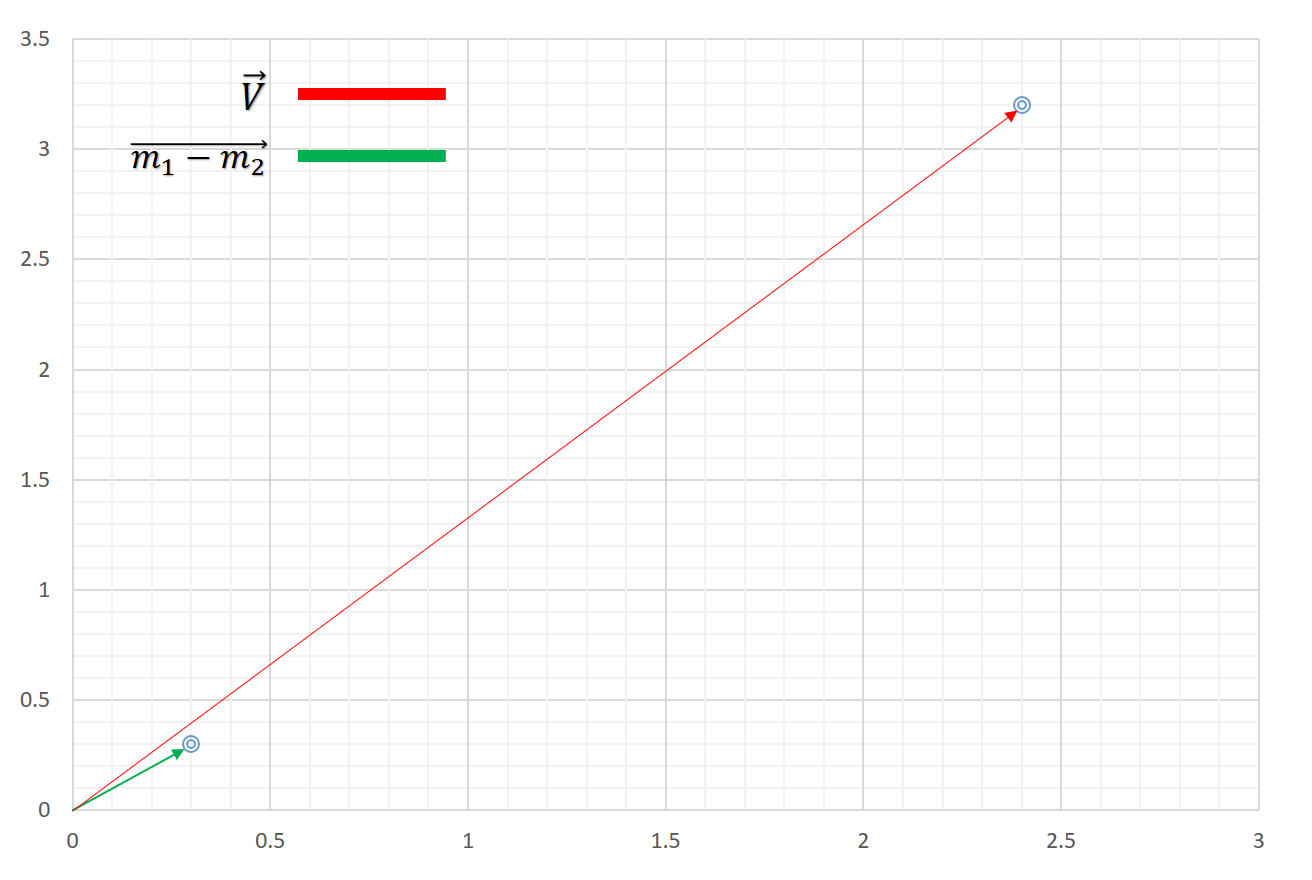
\includegraphics[width=0.7\textwidth]{2_c.PNG}
	\caption{Illustration of FLD Projection Vector and Mean Deviation Vector.}
	\label{pl1}
\end{figure}

(d) In order to perform a principal component analysis on the dataset, we should find the global scatter matrix of our data. In this case, we don't care about the classes and assume the whole data as a single class. Before going further, we have to make sure that all data are decreased by the mean vector value.
$$
	S = 8 *	\renewcommand\arraystretch{1}
	\begin{bmatrix}
	-0.05 & -0.05 & 0.35 & 0.25 & -0.05 & -0.25 & -0.2 & -0.1 \\
	0 & 0.2 & 0.2 & 0.3 & -0.1 & -0.2 & -0.1 & -0.3 \\
	\end{bmatrix} 	\begin{bmatrix}
	-0.05 & 0\\
	-0.05 & 0.2\\
	0.35 & 0.2\\
	0.25 & 0.3\\
	-0.05 & -0.1\\
	-0.25 & -0.2\\
	-0.2 & -0.1\\
	-0.1 & -0.3\\
	\end{bmatrix} = \begin{bmatrix}
	 2.44 & 1.72\\
	 1.72 & 2.56\\
	\end{bmatrix}
$$
In this step, we'll find the eigenvalues of the scatter matrix. We need to solve the following equation.
$$
	\lambda^2 - 5\lambda + 3.29 = 0
$$
which yields the following results:
$$
	\lambda_1 =  4.22 \ \ \ \ \lambda_2 = 0.78
$$
The eigenvector corresponding to the greatest eigenvector is obtained as:
$$
	V = \alpha[1\ \ \ 1.03]^T
$$
where
$$
	\sqrt{\alpha^2 + 1.06\alpha^2} = 1 \ \ \rightarrow \ \ V = [0.69 \ \ 0.71]^T
$$
		\begin{figure}[!h]\centering
	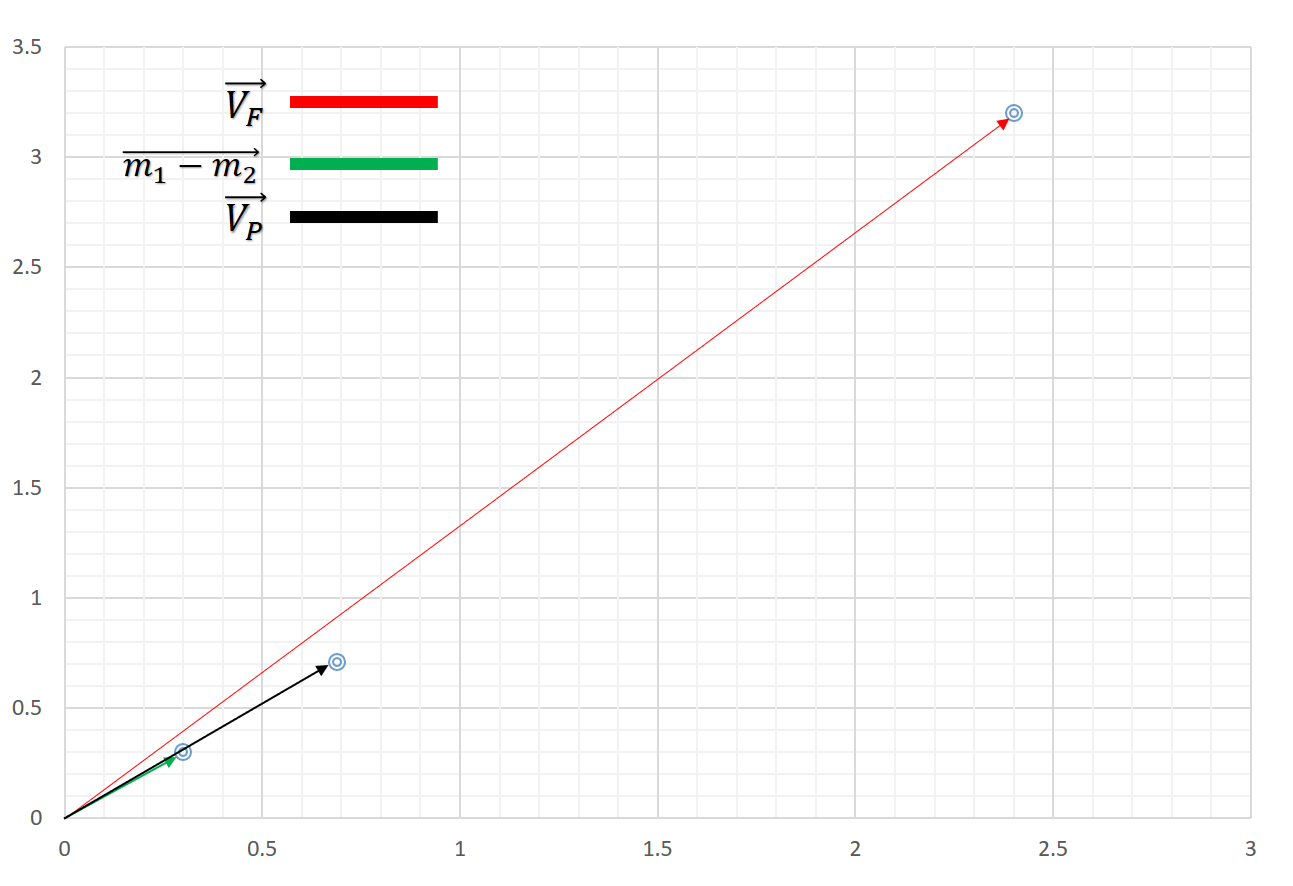
\includegraphics[width=0.65\textwidth]{2_d.PNG}
	\caption{Illustration of PCA Projection Vector.}
	\label{pl1}
\end{figure}

(e) Fisher's vector provides the proper direction in which the classes are mostly separable. However, PCA's vector provides the direction in which the variance of the whole data is maximized and thus useful for representation purposes. Figure 2.3 provides the scatter plot of this phenomenon.
		\begin{figure}[!h]\centering
	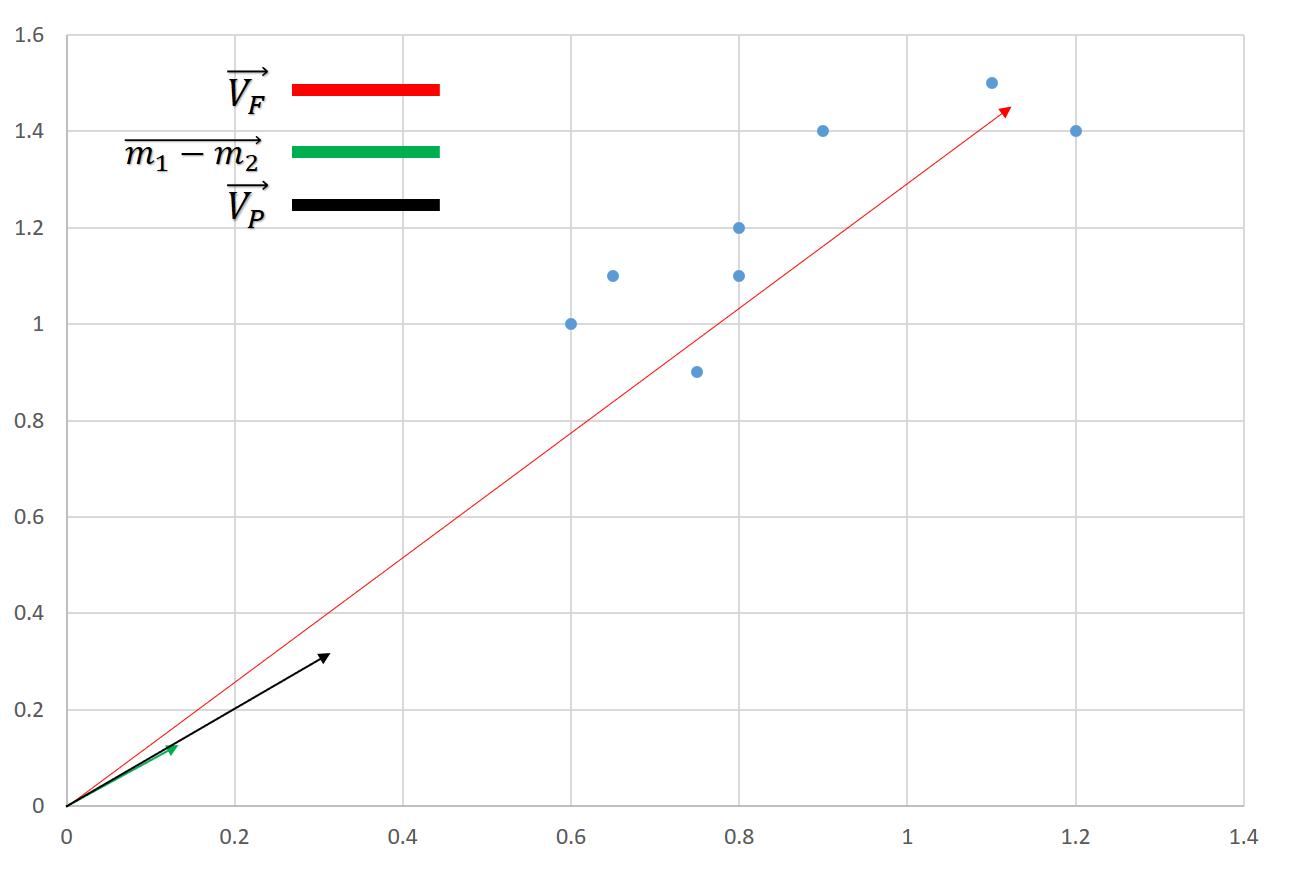
\includegraphics[width=0.65\textwidth]{2_e.PNG}
	\caption{Dataset \& Projection Vectors Using Fisher and PCA Methods.}
	\label{pl1}
\end{figure}

(f) We can use (2.7) to project our samples on a given vector A:
\begin{equation}
	y_i = A^t x_i
\end{equation}
replacing $x_i$ with the test sample and $A^t$ with [2.4 3.2]:
$$
	y = [2.4 \ \ \ 3.2][0.85\ \ \ 1.15]^t = [2.04 \ \ \ 3.68]
$$
\end{document} 



